%%%%%%%%%%%%%%%%%%%%%%%%%%%%%%%%%%%%%%%%%%%%%%%%%%%%%%%%%%%%%%%%%%%%%%%%%%%%%%%%
%%%%%%%%%%%%%%%%%%%%%%%%%%%%%%%%%%%%%%%%%%%%%%%%%%%%%%%%%%%%%%%%%%%%%%%%%%%%%%%%
\documentclass[addpoints,12pt,solution]{exam}
\printanswers
\usepackage{amsmath,amssymb}
\usepackage{comment}
\usepackage{graphicx}
\usepackage{ulem}
\usepackage{paralist}
\usepackage{tabto}
\usepackage{psfrag}
\usepackage{fullpage}
\usepackage{fancybox}
\usepackage{ifthen}
\usepackage{hyperref}
\usepackage{marvosym}
\usepackage{tikz}
\usepackage{amsmath}
\usepackage[ruled,vlined,noresetcount]{algorithm2e}
\usepackage{enumitem}
\usepackage{multirow}
\marksnotpoints


\begin{document}


\hrule
\vspace{1mm}
\noindent 
\begin{center}
{\Large CS6700 : Reinforcement Learning} \\
{\large Written Assignment \#1}
\end{center}
\vspace{1mm}
\noindent 
{\large Intro to RL, Bandits, DP   \hfill Deadline: 23 Feb 2020, 11:55 pm}


%%%%%%%%%%%%%%%%%%%%%%%%%%%%%%%%%%%%%%%%%%%%%%%%%%%%%%%%%%%%%%%%
% Enter name and roll number here
\noindent {\bf Name:} Pragnesh Rana \hfill {\bf Roll number:} ME17S301
%%%%%%%%%%%%%%%%%%%%%%%%%%%%%%%%%%%%%%%%%%%%%%%%%%%%%%%%%%%%%%%%%%
\vspace{2mm}
\hrule

{\small

\begin{itemize}\itemsep0mm
\item This is an individual assignment. Collaborations and discussions are strictly
prohibited.
\item Be precise with your explanations. Unnecessary verbosity will be penalized.
\item Check the Moodle discussion forums regularly for updates regarding the assignment.
\item Type your solutions in the provided \LaTeX template file.
\item \textbf{Please start early.}
\end{itemize}
}

\hrule

\vspace{3mm}




%\gradetable[h][questions]

%%%%%%%%%%%%%%%%%%%%%%%%%%%%%%%%%%%%%%%%%%%%%%%%%%%%%%%%%%%%%%%%%%%%%%%%%%%%%%
%%%%%%%%%%%%%%%%%%%%%%%%%%%%%%%START HERE%%%%%%%%%%%%%%%%%%%%%%%%%%%%%%%%%%%%%%
\begin{questions}
\question[2] You have come across Median Elimination as an algorithm to get $(\epsilon, \delta)-$PAC bounds on the best arm in a bandit problem. At every round, half
of the arms are removed by removing arms with return estimates below
the median of all estimates. How would this work if we removed only
one-fourth of the worst estimated arms instead? Attempt a derivation of
the new sample complexity.

\begin{solution}
%Write solution here
\\
For ($\epsilon,\delta$) PAC algorithm \cite{even2002pac},  \\
Let a' be an arm for which E[R(a')] $<$ $r^{*}$ - $\epsilon$ \\
$\Pr({r_{a'}} > {r_{a^{*}}})$ \\
$ \le P(r_{a'} > E[R(a')]) + \epsilon/2$ or $r^{*} - \epsilon/2$ \\
$ \le P(r_{a'} > E[R(a')]) + \epsilon/2 + r^{*} - \epsilon/2$ \\
$ \le 2 \exp(-(\epsilon/2)^{2} l )$ \\
choosing the $l=\frac{4}{\epsilon}^2 \log \frac{2n}{\delta}{}$ assures that $\Pr(r_{a'}>r_{a}) < \delta/n)$ \\

Now, The failure probability by $E = \{r^{*}_1 < r_1 - \epsilon_1 / 2\}$ \\
$\Pr\{r_{j} \geq r_1 | r_1 \geq - \epsilon /2 \} \leq  \Pr\{r_{j} \geq r_j + \epsilon /2 | r_{1}^* \geq r_1 - \epsilon /2\} \leq \frac{\delta_1}{3}$  

Let $\#bad $ be the number of arms which are not $spdilon_1$-optimal but are empirically better than the best arm. 
$E[\#bad|r_1^{*}  \geq r_1 - \epsilon/2] \leq n\delta_1/3$ \\

$\Pr\{ \#bad \geq n/4 | r_{1}^* \geq r_1 - \epsilon /2 \} \leq \frac{n\delta_1 / 3}{n/4} $ = $ 4 \delta /3$
which shows that prpobability of failure is bunded by $\delta$ \\


Number of samples in $l^{th}$ round is $\frac{4\delta \ln(3/\delta_l) }{\epsilon_i^{2}}$\\

so, \\
$\delta_1 = \delta/2 ; $ $\delta_l = \delta_{l-1}/2 = \delta/2l$ \\
$n_1 = n/2 ; $ $n_l = 3n_{l-1}/4 = (3/4)^{l-1}n$ \\
$\epsilon_1 = \epsilon/2 ; $ $\epsilon_l = 3/4 \epsilon_{l-1} = (3/4)^{l-1} \epsilon/4$ \\

Therefore, \\
$\sum_{l=1}^{\log_2 n} \frac{n_l \ln(3/\delta)}{(\epsilon_{l-1}/2)^2}$ \\
= $4 \sum_{l=1}^{\log_2 n} \frac{(3/4)^{l-1}n \ln(2^l 3/\delta)}{((3/4)^{l-1}\epsilon/4)^2}$ \\
= $64 \sum_{l=1}^{\log_2 n} (4/3)^{l-1} \frac{n }{\epsilon^2}\ln(2^l 3/\delta)$ \\
\textbf{As this series diverges so changing the epsilon,}

= $\epsilon_1^2 = \epsilon^2/16 ; $ $\epsilon_l^2 = (15/16) \epsilon^2_{l-1} = (15/16)^{l-1} \epsilon^2/16$ \\
so, \\
= $4 \sum_{l=1}^{\log_2 n} \frac{(3/4)^{l-1}n \ln(2^l 3/\delta)}{((15/16)^{l-1}\epsilon^2/16)}$ \\
= $64 \sum_{l=1}^{\log_2 n} (4/5)^{l-1} \frac{n }{\epsilon^2}\ln(2^l 3/\delta)$ \\
= $64 \frac{n }{\epsilon^2} \sum_{l=1}^{log_2n} (4/5)^{l-1} [l\ln(2^l) + \ln(3) + \ln(1/\delta)]$ \\
$\leq$  $64 \frac{n }{\epsilon^2} \ln(1/\delta) \sum_{l=1}^{\infty} (4/5)^{l-1} [lC' + C ]$ \\ 
$\leq$  $\mathcal{O}(\frac{n \ln(1/\delta) }{\epsilon^2})$

\end{solution}

\question[3] Consider a bandit problem in which you know the set of expected payoffs for pulling various arms, but you do not know which arm maps to which expected payoff. For example, consider a 5 arm bandit problem and you know that the arms 1 through 5 have payoffs 3.1, 2.3, 4.6, 1.2, 0.9, but not necessarily in that order. Can you design a regret minimizing algorithm that will achieve better bounds than UCB? What makes you believe that it is possible? What parts of the analysis of UCB will you modify to achieve better bounds?
\begin{solution}
%Write solution here 
\\
1. yes, it is possible to design the regret minimizing algorithm toa achiee better bound than UCB.

2. 
\textbf{How UCB works?} \\
- A machine is randomly picked and Each machie have (uniform) same initial confidence interval and success distribution.  \\
- Based on the reward, the confidence interval shifts either toward or away from the actual succesive distribution which eventually converges or due to exploration and results in the reductionn of the upper bound value of the confidence interval.\\
- Based on the updated upper cofidence boundof each machines, the one with highest is chosen to explore in the next round. \\
\textbf{CHANGE:} \cite{stocha}\\
\textbf{(LUCB++)} : Rather than picking the best arm, it is prefreable to pick K-best arms. Finding the top-K arms required k and k+1 best arm, which makes confident that the worst arm in the top-K set is better than the best arm in the set of remaining arms. \\

3.\textbf{Modification in UCB:} \\
UCB only picks the best arm but in new algo K best are picked. By preceding in this manner by creating and refining estimates of the expected reward of the k-th and k+1-th best arm, termites the algo once the worst arm in the top k set is better than best arm in the set of remaining with desired confidence. 


\end{solution}

\question[3]Suppose you face a 2-armed bandit task whose true action values change randomly from time step to time step. Specifically, suppose that, for any time step, the true values of actions 1 and 2 are respectively 0.1 and 0.2 with probability 0.5 (case A), and 0.9 and 0.8 with probability 0.5 (case B). 

\begin{enumerate}[label=(\alph*)]
    \item (1 mark) If you are not able to tell which case you face at any step, what is the best expectation of success you can achieve and how should you behave to achieve it?
\begin{solution}
%Write solution here
1. As we don't know any detail priori, one cannot estimate individual detail for case A and B. The best approach to find out \textbf{best expectation such that which maximize the reward in combinations} for any case, means find optimal case such away that combination of both case is toward maximum reward and.\\
Possible cases are \cite{sutton2018reinforcement}:\\
\textbf{$C_1 = 0.1 *0.5 + 0.9*0.5 = 0.5$} \textbf{Best} \\
$C_2 = 0.1 *0.5 + 0.8*0.5 = 0.45$\\

\textbf{$C_4 = 0.2 *0.5 + 0.8*0.5 = 0.5$} \textbf{due to possible dependency} 


	
 For given case maximum expected reward is 0.55. but out of  first two case maximum expected reward is 0.5 and as action independence is not known so, C1 will preferred. \\
 
  Second case is selected such away that which does not include any detail from case-1 as dependecy of actions not known. \\
  
  To optimize reward in any case we prefer to select action in such way that selection of any case leads to maximize the for other case also. \\
  
 For given case, estimate for two case is same in C1 and C4. The best expectation of success is 0.5 which can be achived by selecting action randomly at eah step.\\

$C_1 = 0.5 * 0.1  + 0.5 * 0.9 = 0.5$ \\
$C_4 = 0.5*0.2 +0.5*0.8 =0.5$ \\

\end{solution}
    
    \item (2 marks) Now suppose that on each step you are told whether you are facing case A or case B (although you still don’t know the true action values). This is an associative search task. What is the best expectation of success you can achieve in this task, and how should you behave to achieve it?
\begin{solution}
%Write solution here
Associative search task involves trial and error learning in the form of search for the best arm.\ref{sutto}.
If we know we are either facing case A or case B then we can learn the best action by considering each case independent to each other. \\
so, possible combinations are, \\
$C_1 = 0.1 *0.5 + 0.9*0.5 = 0.5$\\
$C_2 = 0.1 *0.5 + 0.8*0.5 = 0.45$\\
$C_3 = 0.2 *0.5 + 0.9*0.5 = 0.55$\\
$C_4 = 0.2 *0.5 + 0.8*0.5 = 0.5$\\


Out of this possible cambination only that action is preferred which gives maximum reward which is C3,\\
$C_3 = 0.2 *0.5 + 0.9*0.5 = 0.55$\\

\end{solution}
\end{enumerate}
 




\question[5]Many tic-tac-toe positions appear different but are really the same because of symmetries. 
\begin{enumerate}[label=(\alph*)]
    \item (2 marks) How might we amend the learning process described above to take advantage of this? In what ways would this change improve the learning process? 
    
\begin{solution}
%Write solution here
In Tic-Tac-Toe, 4 axis of symmetry(two central axis and two diaonal axis) is possible. Using this 4 axis symmetry, the board can be fold down to a quarter of the original size.\\
Advantage of symmetry will reduce the memory requirement and increase the performance of the algorithm.
\end{solution}

    \item (1 mark) Suppose the opponent did not take advantage of symmetries. In that case, should we? Is it true, then, that symmetrically equivalent positions should necessarily have the same value? 
    
\begin{solution}
%Write solution here
If opponent is not using advantage of symmetry then overall performance will become worse.  \\

Example:  Out of all positionn if opponent always played correct in one corner position denotes that player never took advantage symmetry. Which also shows that if you take advantage of symmetry then symmetrical equivalent position doesn't hold the same value in a multi-player game.

\end{solution}

    \item (2 marks) Suppose, instead of playing against a random opponent, the reinforcement learning algorithm described above played against itself, with both sides learning. What do you think  would happen in this case? Would it learn a different policy for selecting moves? 
    
\begin{solution}
%Write solution here
If player plays against itself then player will continue to adapt untill it reaches an equillibrium, which might be either fixed or cyclic. \\
After equillbrium it can learn higher skill against fixed opponent but it may happen that it may take wrong paths while reacting to itself.\\


\end{solution}

\end{enumerate}

\question[1]Ego-centric representations are based on an agent's current
position in the world. In a sense the agent says, I don’t care where
I am, but I am only worried about the position of the objects in the
world relative to me. You could think of the agent as being at the origin
always. Comment on the suitability (advantages and disadvantages)
of using an ego-centric representation in RL.

\begin{solution}
%Write solution here

When agent is performing egonocentric leraning then it distinguishes situation based on it's immediate surrounding environment. For the case of cliff, learning Q-values where each state is set of immediate neighbours. \cite{ego} \\
Advantage: \\
Due to immediate neighbour \textbf{minimal number of death will be observed.}

Disadvatage:\\
- Due to immediate states number of success will be consistent or low as while avoiding cliffs it goes to other states randomly.
- With increase in size of the area, wins reduces.

\end{solution}

\question[2] Consider a general MDP with a discount factor of $\gamma$.
For this case assume that the horizon is infinite. Let $\pi$ be a policy and $V^{\pi}$ be the corresponding value function. Now suppose we have a new
MDP where the only difference is that all rewards have a constant $k$ added to them. Derive the new value function $V^{\pi}_{new}$ in terms of $V^{\pi},\ c$ and $\gamma$.

\begin{solution}\\
%Write solution here
It is given that \\
$v^{\pi}_{old}(s_i) = v^{\pi}(s_i) = \sum_{t=0}^{\infty} \gamma^t r_t $ \\

but by adding constant to the reward obtain value fucntion is,\\

$v^{\pi}_{new}(s_i) = \sum_{t=0}^{\infty} \gamma^t (r_t + c) $ \\
$v^{\pi}_{new}(s_i) = \sum_{t=0}^{\infty} \gamma^t r_t + \sum_{t=0}^{\infty} \gamma^t c$ \\
$v^{\pi}_{new}(s_i) = v^{\pi}_{old}(s_i) + \sum_{t=0}^{\infty} \gamma^t c$ \\
\end{solution}


\question[4] An $\epsilon$-soft policy for a MDP with state set $\mathcal{S}$ and action set $\mathcal{A}$ is any policy that satisfies \[\forall a\in \mathcal{A}, \forall s \in \mathcal{S}: \pi(a|s)\geq \frac{\epsilon}{|\mathcal{A}|}\]
Design a stochastic gridworld where a deterministic policy will produce
the same trajectories as a $\epsilon$-soft policy in a deterministic
gridworld. In other words, for every trajectory under the same policy, the
probability of seeing it in each of the worlds is the same. By the same policy I mean that in the stochastic gridworld, you have a deterministic policy and in the deterministic gridworld, you use the same policy, except for $\epsilon$ fraction of
the actions, which you choose uniformly randomly. 
\begin{enumerate}[label=(\alph*)]
\item (2 marks) Give the complete specification of the world.


\begin{solution}
%Write solution here
\textbf{Grid World:} \\

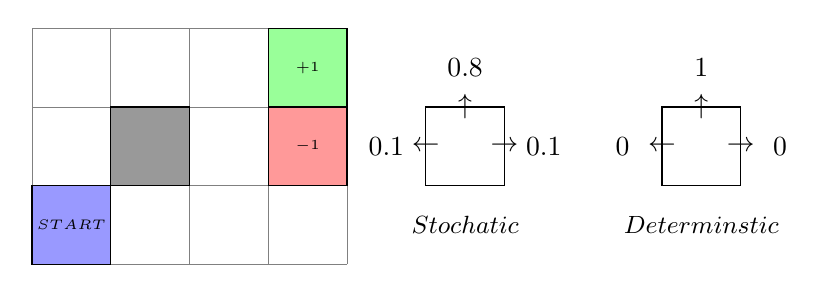
\begin{tikzpicture}
\draw[step=1cm,gray,very thin] (0,0) grid (4,3);
\filldraw[fill=blue!40!white, draw=black] (0,0) rectangle (1,1) ;
\draw (0.5,0.5)node {\tiny $START$} ;
\filldraw[fill=black!40!white, draw=black] (1,1) rectangle (2,2) ;
\filldraw[fill=red!40!white, draw=black] (3,1) rectangle (4,2) ;
\filldraw[fill=green!40!white, draw=black] (3,2) rectangle (4,3) ;
\draw (3.5,1.5)node {\tiny $-1$} ;
\draw (3.5,2.5)node {\tiny $+1$} ;

%stochastic
\filldraw[fill=white!40!white, draw=black] (5,1) rectangle (6,2) ;
\node at (5.5,2) {$\large \uparrow$ };
\node at (5.5,2.5) {$0.8$ };
\node at (5,1.5) {$\large \leftarrow$ };
\node at (4.5,1.5) {$0.1$ };
\node at (6,1.5) {$\large \rightarrow$ };
\node at (6.5,1.5) {$0.1$ };
\draw (5.5,0.5) node  {\small $Stochatic$};

%determinstic
\filldraw[fill=white!40!white, draw=black] (8,1) rectangle (9,2) ;
\node at (8.5,2) {$\large \uparrow$ };
\node at (8.5,2.5) {$1$ };
\node at (8,1.5) {$\large \leftarrow$ };
\node at (7.5,1.5) {$0$ };
\node at (9,1.5) {$\large \rightarrow$ };
\node at (9.5,1.5) {$0$ };
\draw (8.5,0.5) node  {\small $Determinstic$};
\end{tikzpicture}\\
\\

 In the maze like problem : \\
 - agent lives in grid \\
 - wall blocks agents path \\
 
 
With certain probability agent moves in certain direction(let's say with probability 0.8 agent moves in north direcion and with probability 0.1 agent moves in east and west direction) \\

Agents recives 'small'reward after each time step. After complition of successful attempt it receives the final reward $\pm 1 $.\\


\textbf{Determinstic World:} The set of states of the environment is composed of each cell of the grid. Set of action is composed of \{left,right,up,down\} and \textbf{given stat $s \in S, \space \pi(s)$ with probability 1 always takes same action for given policy.} If policy changes there might be chance of change of action.\\



\textbf{Stochastic World :}  Set of action is composed of \{left,right,up,down\} and \textbf{given stat $s \in S, \space \pi(s)$ the agent move to next state with certain probability in next time-step .} In short, for same state and same policy there might be some chace that agent will select different state every next time. \\

For both cases, the agent uses determinstic policy. \\
- In stochastic grid world, determinstic policy is used so randomness in selection of state will be reduced and ultimately it picks the optimal path by updating the deterministic policy. \\

-In determinstic grid world, it also uses deterministic policy with $\epsilon$-soft policy in which it follows the specific but $\epsilon$ time it randomly picked another state with uniform probability and try to update the policy and eventually converge to the final optimal policy which will be same above obtain policy and path. 
\end{solution}


\item (2 marks) Will SARSA on the two worlds converge to the same policy? Justify.

\begin{solution}
%Write solution here
\\
Yes, SARSA in the two world will converge to the same policy.\cite{on}\\

SARSA(s,a,r,s',a') is on-policy reinforcement learning algorithm which estimates the value of policy being followed. It uses the action perfomed by the current policy to learn Q-value.

$Q(s_t,a_t) = Q(s_t,a_t) + \alpha (r_{t+1} + \gamma Q(s_{t+1},a_{t+1}) - Q(s_t,a_t))$

SARSA accounts the current exploration policy which may be greedy with random steps.\\
Being greedy with random steps, it behaves like $\epsilon$-greedy deterministic policy. It will find a policy that is optimal, taking into account the exploration inherent in the policy. 
\end{solution}

\end{enumerate}

\question[7]You receive the following letter:\\
Dear Friend, Some time ago, I bought this old house, but found it to be haunted by
ghostly sardonic laughter. As a result it is hardly habitable. There is hope, however,
for by actual testing I have found that this haunting is subject to certain laws, obscure
but infallible, and that the laughter can be affected by my playing the organ or burning
incense. In each minute, the laughter occurs or not, it shows no degree. What it will
do during the ensuing minute depends, in the following exact way, on what has been
happening during the preceding minute: Whenever there is laughter, it will continue in
the succeeding minute unless I play the organ, in which case it will stop. But continuing
to play the organ does not keep the house quiet. I notice, however, that whenever I
burn incense when the house is quiet and do not play the organ it remains quiet for the
next minute. At this minute of writing, the laughter is going on. Please tell me what
manipulations of incense and organ I should make to get that house quiet, and to keep
it so.\\
Sincerely,\\
At Wits End
\begin{enumerate}[label=(\alph*)]
    \item (3 marks) Formulate this problem as an MDP (for the sake of uniformity, formulate it as a
continuing discounted problem, with $\gamma= 0.9$. Let the reward be +1 on any transition
into the silent state, and -1 on any transition into the laughing state.) Explicitly give the
state set, action sets, state transition, and reward function.
\begin{solution}
%Write solution here
\\
\textbf{State set: } \{L,Q\} 
where,\\
L indicates laughter in the room \\
Q indicates Quite \\

\textbf{Action set:} $\{O\wedge I,O\wedge \neg I\, \neg O \wedge I, \neg O \wedge \neg I \}$

where,\\
O denotes to the playing the organ  \\
I denotes burning incense \\
$\wedge$ denotes 'AND' \\
$\neg$ denotes 'Not' \\

Assuming determinstinc transition and reward following states are possible,\\

	\begin{tabular}{cccc}
			\hline
			\multicolumn{3}{|c|}{State Transition}                                                              & \multicolumn{1}{c|}{\multirow{2}{*}{Reward}} \\ \cline{1-3}
			\multicolumn{1}{|c|}{Current state} & \multicolumn{1}{c|}{Action} & \multicolumn{1}{c|}{Next state} & \multicolumn{1}{c|}{}                        \\ \hline
			\multicolumn{1}{|c|}{L}              & \multicolumn{1}{c|}{$ O\wedge I$}       & \multicolumn{1}{c|}{Q}           & \multicolumn{1}{c|}{+1}                        \\ \hline
			\multicolumn{1}{|c|}{Q}              & \multicolumn{1}{c|}{$O\wedge I$ }       & \multicolumn{1}{c|}{Q}           & \multicolumn{1}{c|}{+1}                        \\ \hline
			\multicolumn{1}{|c|}{Q}              & \multicolumn{1}{c|}{$O\wedge \neg I$}       & \multicolumn{1}{c|}{L}           & \multicolumn{1}{c|}{-1}                        \\ \hline
			\multicolumn{1}{|c|}{Q}              & \multicolumn{1}{c|}{$\neg O \wedge I$}       & \multicolumn{1}{c|}{Q}           & \multicolumn{1}{c|}{+1}                        \\ \hline
			\multicolumn{1}{|c|}{Q}                & \multicolumn{1}{c|}{$\neg O \wedge \neg I$}        & \multicolumn{1}{|c|}{L}            & \multicolumn{1}{c|}{-1}           \\ \hline             
		\end{tabular}

\end{solution}

    \item (2 marks) Starting with simple policy of \textbf{always} burning incense, and not playing organ, perform a couple of policy iterations.
\begin{solution}
%Write solution here
\\
\textbf{policy : }\\
$\pi\{a|\text{always burning incense , not playing organ\}} $ \\
\begin{itemize}
	\item if state = Laughter 
	\subitem	$\tab\pi\{a|\text{always burning incense , play organ \}} $ $\rightarrow$ state: Laughter $\rightarrow $ Quite 
	\subitem if state = Quite
	\subitem $\tab\pi\{a|\text{always burning incense , do not play organ \}}$ Quite  $\rightarrow$ Quite 
	
	
	\item if state = Quite 
	\subitem $\pi\{a|\text{always burning incense , play organ \}} \rightarrow $ state : Quite $\rightarrow$ Noise
	 \subitem if state = Quite 
	\subitem $\pi\{a|\text{always burning incense , do not play organ \}} $ state: Quite $\rightarrow$ Quite\\	
	
	
\end{itemize}

	

\end{solution}
    
    \item (2 marks) Finally, what is your advice to "At Wits End"?
\begin{solution}
%Write solution here
\\
It is advisable to play organ when there is laughter \\
and if room is quite, do not play the organ and burn incense. 
\end{solution}
    
    
\end{enumerate}

\question[4] Consider the task of controlling a system when the control actions are delayed. The control agent takes an action on observing the state at time $t$. The action is applied to the system at time $t + \tau$. The agent
receives a reward at each time step.
\begin{enumerate}[label=(\alph*)]
\item (2 marks)What is an appropriate notion of return for this task?
\begin{solution}
%Write solution here
For delayin control action and delayed reward, any approach which learns Q should work fine with delayed reward.  Monte Carlo Control, SARSA, Q-learning, DQN and all other variants are in theory capable of learning the delayed reward.\cite{ans}
\textbf{Return:} \\
New Return  = old return +discounted factor *  temporal difference 

$Q(s_t,a_t) \leftarrow Q(s_t,a_t) + \alpha [r_t + \gamma Q(s_{t+\tau},a_{t+\tau} - Q(s_t,a_t))]$

generally \textbf{return in monte carlo} is obtained by,\\
$G_t = R_{t+\tau} + \gamma R_{t+2 \tau} + ... = \sum_{k=1}^{\infty} \gamma^k R_{t+k \tau }$

where, \\
$G_t$  = total discouter reward \\
$\gamma$ = discount factor\\
$R_{t+\tau }$ = reward at time t+$\tau$ \\

which can be simplified as, \\
$G_t = R_{t+1} + \gamma R_{t+1} + ...$ \\
Further \\
$G_t = R_{t+1} + \gamma G_{t+1}$ \\
\textbf{$G_t \approx R_{t+1} + \gamma v_(s_{t+1})$ } \cite{TD0}

\end{solution}
\item (2 marks) Give the TD(0) backup equation for estimating the value function of a given policy.
\begin{solution}
%Write solution here
\\
Value function is generally given as\cite{TD0} ,\\
$v_{new}(s) = v_{old}(s) + \alpha [G_t -v_{old}(s) ]$

now, replacing the target return using above obtained result,\\
policy can be obtain as,\\
$v_{new}(s_t) = v{old}(s_t) + \alpha [ R_{t+1} + \gamma v_{old}(s_{t+1}) -v_{old}(s_t) ]$

\end{solution}
\end{enumerate}
\end{questions}
\newpage
%%
%% Following citation commands can be used in the body text:
%% Usage of \cite is as follows:

%%   \cite{key}          ==>>  [#]
%%   \cite[chap. 2]{key} ==>>  [#, chap. 2]
%%   \citet{key}         ==>>  Author [#]

%% References with bibTeX database:
\bibliographystyle{ieeetr}
\bibliography{biblio.bib}		
%%%%%%%%%%%%%%%%%%%%%%%%%%%%%%%%%%%%%%THE END%%%%%%%%%%%%%%%%%%%%%%%%%%%%%%%%%%%

\end{document}